\documentclass[12pt, a4paper]{report}

%%%%%%%%%%%%%%%%%%%%%%%%%%%%
% PAGE LAYOUT
%%%%%%%%%%%%%%%%%%%%%%%%%%%%
\usepackage[left=0.8in, right=0.8in, top=1in, bottom=1in]{geometry}
\usepackage[utf8]{inputenc}
\usepackage{parskip}        % No paragraph indents
\usepackage{multicol}
\usepackage{array}
\usepackage{longtable}
\usepackage{multirow}
\usepackage{tabularx}
\usepackage{booktabs}       % Professional tables
\usepackage{float}          % Image/table placement
\usepackage{graphicx}       % Images
\usepackage{subcaption}
\usepackage{enumitem}       % List formatting
\usepackage{comment}        % Multi-line comments
\usepackage{import}
\usepackage{xifthen}
\usepackage{pdfpages}
\usepackage{transparent}
\usepackage{titlesec}       % Section formatting
\usepackage{titletoc}
\usepackage[version=4]{mhchem}
\usepackage{chngcntr}
\usepackage{fancyhdr}       % Headers and footers
\usepackage{varwidth}
\usepackage{etoolbox}
\usepackage{xcolor}
\usepackage{nameref}
\usepackage{caption} % Added for \captionof outside floats
\usepackage{markdown}
\usepackage{authblk} % for adding affiliations
\usepackage{dirtree}
\usepackage{microtype}      % ADDED: better justification/kerning, no visual surprises, safe default for notes
%%%%%%%%%%%%%%%%%%%%%%%%%%%%
% MATH — order matters here
%%%%%%%%%%%%%%%%%%%%%%%%%%%%
\usepackage{amsthm}             % Must come BEFORE newpxmath (both define \openbox)
\usepackage{amsmath, mathtools} % Core math environments
\usepackage[varbb]{newpxmath}   % Load after amsthm/amsmath
\usepackage{amssymb}            % Extra math symbols
\usepackage{mathrsfs}           % \mathscr script font
\usepackage{bm}                 % Bold math symbols
\usepackage{xfrac}              % \sfrac
\usepackage{siunitx}            % SI units
\usepackage{cancel}             % Strikeout in equations
\usepackage{systeme}            % Systems of equations

% Allow display-math breaks across pages
\allowdisplaybreaks

% Extra spacing in multiline environments
\setlength{\jot}{10pt}

%%%%%%%%%%%%%%%%%%%%%%%%%%%%
% SYMBOLS (selective — avoids "too many symbol fonts")
%%%%%%%%%%%%%%%%%%%%%%%%%%%%
\usepackage{gensymb}            % \degree, \celsius, etc.
% wasysym removed: declare only what you need to avoid font-slot overflow.
% If you need \Square / \Circle etc., uncomment the line below:
% \usepackage[only,Square,Circle,diameter,checked]{wasysym}

%%%%%%%%%%%%%%%%%%%%%%%%%%%%
% FONTS & LANGUAGE
%%%%%%%%%%%%%%%%%%%%%%%%%%%%
\usepackage{fontspec}

% Devanagari MT only ships with macOS. Fall back to another Devanagari font
% when it is missing (e.g. on Linux/CI) so the document builds anywhere.
% \dn is not used in the text yet, so no font at all is also acceptable.
\IfFontExistsTF{Devanagari MT}
  {\newfontfamily\hindi[Script=Devanagari]{Devanagari MT}}
  {\IfFontExistsTF{Noto Sans Devanagari}
     {\newfontfamily\hindi[Script=Devanagari]{Noto Sans Devanagari}}
     {\newcommand{\hindi}{}}}

%%%%%%%%%%%%%%%%%%%%%%%%%%%%
% LINKS & REFERENCES
%%%%%%%%%%%%%%%%%%%%%%%%%%%%
\usepackage{bookmark}
\usepackage{hyperref,theoremref}
\usepackage{url}
\usepackage{cleveref}        % ADDED: must load after hyperref. Needed now that
                              % theorem/corollary/prop/claim/etc. no longer carry
                              % an automatic tcbtheorem label prefix — \cref{th:foo}
                              % will print "Theorem 1.1" etc. automatically.

\hypersetup{
    colorlinks = true,
    linkcolor  = black,
    filecolor  = magenta,
    urlcolor   = secondaryBlue,
}

% Names cleveref uses for each environment (edit freely)
\crefname{theorem}{Theorem}{Theorems}
\crefname{corollary}{Corollary}{Corollaries}
\crefname{prop}{Proposition}{Propositions}
\crefname{claim}{Claim}{Claims}
\crefname{defn}{Definition}{Definitions}
\crefname{property}{Property}{Properties}
\crefname{qs}{Question}{Questions}
\crefname{remark}{Remark}{Remarks}
\crefname{example}{Example}{Examples}

%%%%%%%%%%%%%%%%%%%%%%%%%%%%
% COLOR DEFINITIONS
%%%%%%%%%%%%%%%%%%%%%%%%%%%%
\usepackage[table]{xcolor}

\definecolor{primaryBlue}   {RGB}{0, 51, 102}
\definecolor{myy}{RGB}{0, 102, 204} % Defines 'myy' as a specific blue (Red, Green, Blue values)
\definecolor{secondaryBlue} {RGB}{70, 130, 180}
\definecolor{doc}           {RGB}{0, 60, 110}
\definecolor{myg}           {RGB}{56, 140, 70}
\definecolor{myb}           {RGB}{45, 111, 177}
\definecolor{myr}           {RGB}{199, 68, 64}
\definecolor{myp}           {RGB}{197, 92, 212}
\definecolor{myred}         {RGB}{127, 0, 0}
\definecolor{mygr}          {HTML}{2C3338}
\definecolor{notesgreen}    {RGB}{0, 162, 0}
\definecolor{headergray}    {RGB}{220, 220, 220}
\definecolor{myo}{RGB}{255, 127, 14}
\definecolor{headGray}      {HTML}{334155}
\definecolor{boxFill}       {RGB}{245, 240, 225}
% NOTE: mytheorembg/mytheoremfr/mypropbg/mypropfr/myqsfr/myexercisebg/myexercisefg
% were only used by the old boxed theorem/corollary/prop/claim/qs environments.
% Now that those are plain (unboxed) amsthm environments, these colors are
% unused. Left them defined in case you want them for something else later —
% delete if you don't need them.
\definecolor{mytheorembg}   {HTML}{F2F2F9}
\definecolor{mytheoremfr}   {HTML}{00007B}
\definecolor{myqsfr}        {HTML}{983b0f}
\definecolor{mypropbg}      {HTML}{f2fbfc}
\definecolor{mypropfr}      {HTML}{191971}
\definecolor{myexercisebg}  {HTML}{F2FBF8}
\definecolor{myexercisefg}  {HTML}{88D6D1}

%%%%%%%%%%%%%%%%%%%%%%%%%%%%
% TCOLORBOX
%%%%%%%%%%%%%%%%%%%%%%%%%%%%
\usepackage[most,many,breakable]{tcolorbox}
\tcbuselibrary{theorems,skins,hooks}

%==============================================================
% THEOREM-LIKE ENVIRONMENTS
% Unified as plain, lightweight amsthm environments (bold head,
% italic body, "." after the head, numbered within section).
% "note" is the only environment kept as a colored tcolorbox,
% since it plays a visually distinct role (a callout, not a
% mathematical statement).
%
% Usage is the standard amsthm pattern for every environment below:
%     \begin{theorem}[Optional title]\label{th:my-label}
%         ...
%     \end{theorem}
% Reference with \cref{th:my-label} (from cleveref, loaded above)
% to get "Theorem 1.1" automatically.
%
% Suggested label-prefix convention (manual, since these are plain
% amsthm environments and no longer auto-prefix labels for you):
%   theorem   -> th:...
%   corollary -> cor:...
%   prop      -> prop:...
%   claim     -> cl:...
%   defn      -> def:...
%   property  -> pty:...   (changed from "prop:" to avoid colliding
%                            with Proposition's "prop:" prefix)
%   qs        -> qs:...
%   remark    -> rem:...
%   example   -> ex:...
%==============================================================
\newtheoremstyle{engnotes}
    {10pt}{10pt}            % space above / below
    {\itshape}              % body font
    {}                       % indent amount
    {\bfseries\sffamily}    % head font
    {.}                      % punctuation after head
    {.5em}                   % space after head
    {}                       % head spec (default: "Name N. (title)")

\theoremstyle{engnotes}
\newtheorem{theorem}{Theorem}[section]
\newtheorem{corollary}{Corollary}[section]
\newtheorem{prop}{Proposition}[section]
\newtheorem{claim}{Claim}[section]
\newtheorem{defn}{Definition}[section]
\newtheorem{property}{Property}[section]
\newtheorem{qs}{Question}[section]
\newtheorem{remark}{Remark}[section]
\newtheorem{example}{Example}[section]
\newtheorem{lemma}{Lemma}[section]

%--------------------------------
% Note box (kept as-is: the one deliberately "loud" callout box)
%--------------------------------
\usepackage{pifont} % Fixes \ding undefined control sequence
\usetikzlibrary{arrows.meta, positioning} % Fixes 'Stealth' arrow error
\usetikzlibrary{arrows,calc,shadows.blur}
\tcbuselibrary{skins}

\newtcolorbox{note}[1][]{
    enhanced jigsaw,
    colback  = gray!20!white,
    colframe = gray!80!black,
    size     = small,
    boxrule  = 1pt,
    title    = \textbf{Note:-},
    halign title  = flush center,
    coltitle      = black,
    breakable,
    drop shadow   = black!50!white,
    attach boxed title to top left = {
        xshift = 1cm,
        yshift = -\tcboxedtitleheight/2,
        yshifttext = -\tcboxedtitleheight/2
    },
    minipage boxed title = 1.5cm,
    boxed title style = {
        colback  = white,
        size     = fbox,
        boxrule  = 1pt,
        boxsep   = 2pt,
        underlay = {
            \coordinate (dotA) at ($(interior.west) + (-0.5pt,0)$);
            \coordinate (dotB) at ($(interior.east) + (0.5pt,0)$);
            \begin{scope}
                \clip (interior.north west) rectangle ([xshift=3ex]interior.east);
                \filldraw [white, blur shadow={shadow opacity=60, shadow yshift=-.75ex},
                rounded corners=2pt]
                (interior.north west) rectangle (interior.south east);
            \end{scope}
            \begin{scope}[gray!80!black]
                \fill (dotA) circle (2pt);
                \fill (dotB) circle (2pt);
            \end{scope}
        },
    },
    #1,
}

%%%%%%%%%%%%%%%%%%%%%%%%%%%%
% TIKZ / PGFPLOTS / FOREST
%%%%%%%%%%%%%%%%%%%%%%%%%%%%
\usepackage{tikz}
\usetikzlibrary{trees,shadows,positioning}
\usepackage[edges]{forest}
\usepackage{pgfplots}
\pgfplotsset{compat=1.18}

%%%%%%%%%%%%%%%%%%%%%%%%%%%%
% ALGORITHMS
%%%%%%%%%%%%%%%%%%%%%%%%%%%%
\usepackage{algorithm}
\usepackage{algpseudocode}

%%%%%%%%%%%%%%%%%%%%%%%%%%%%
% CODE LISTINGS
%%%%%%%%%%%%%%%%%%%%%%%%%%%%
\usepackage{minted}

\fvset{showspaces}
\renewcommand\FancyVerbSpace{\textcolor{white}{\char32}}

\setminted{
    bgcolor    = gray!12,
    fontfamily = tt,
    linenos    = true,
    tabsize    = 4,
}

\setminted[python]{
    linenos=true,
    frame=lines,
    python3=true,
    breaklines=true,
}

%%%%%%%%%%%%%%%%%%%%%%%%%%%%
% HEADERS & FOOTERS
%%%%%%%%%%%%%%%%%%%%%%%%%%%%
\setlength{\headheight}{14pt}
\pagestyle{fancy}
\fancyhf{}

\newcommand{\SubjectName}{}
\newcommand{\UnitName}{}
\newcommand{\SetHeader}[2]{
    \renewcommand{\SubjectName}{#1}
    \renewcommand{\UnitName}{#2}
}

\rhead{\textcolor{headGray}{\SubjectName}}
\lhead{%
    \begin{varwidth}{0.5\textwidth}
        \raggedright
        \color{headGray}
        \UnitName
    \end{varwidth}%
}
\rfoot{Page \thepage}

\title{\textbf{\Huge \UnitName}}

%%%%%%%%%%%%%%%%%%%%%%%%%%%%
% CUSTOM COMMANDS
%%%%%%%%%%%%%%%%%%%%%%%%%%%%
\setlength{\parindent}{1cm}
\setlist[itemize]{itemsep=0.2em, topsep=0.2em}

% Math sets
\newcommand\N{\ensuremath{\mathbb{N}}}   % fixed: was \bb{N}
\newcommand\R{\ensuremath{\mathbb{R}}}
\newcommand\Z{\ensuremath{\mathbb{Z}}}
\newcommand\Q{\ensuremath{\mathbb{Q}}}
\newcommand\C{\ensuremath{\mathbb{C}}}
\renewcommand\O{\ensuremath{\emptyset}}
\newcommand{\br}{\mathbf{r}}

% Paired delimiters
\DeclarePairedDelimiter{\abs} {\lvert}  {\rvert}
\DeclarePairedDelimiter{\norm}{\lVert}  {\rVert}
\DeclarePairedDelimiter{\ceil}{\lceil}  {\rceil}
\DeclarePairedDelimiter{\floor}{\lfloor}{\rfloor}
\DeclarePairedDelimiter{\round}{\lfloor}{\rceil}

\DeclareSIUnit{\dBm}{dBm}
\DeclareSIUnit\month{mo}
\DeclareSIUnit\year{yr}
\DeclareSIUnit{\pound}{lb}

% ADDED: common operators used constantly in engineering-grad math
% (optimization / linear algebra). Remove any you don't need.
\DeclareMathOperator*{\argmax}{arg\,max}
\DeclareMathOperator*{\argmin}{arg\,min}
\DeclareMathOperator{\tr}{tr}
\DeclareMathOperator{\rank}{rank}
\DeclareMathOperator{\diag}{diag}
\DeclareMathOperator{\sgn}{sgn}
\DeclareMathOperator{\dom}{dom}
\DeclareMathOperator{\spann}{span}
\DeclareMathOperator{\dist}{dist}
% Misc
\newcommand\contra{\scalebox{1.5}{$\lightning$}}
\newcommand{\dn}[1]{{\hindi #1}}
\newcommand{\textbi}[1]{\textbf{\textit{#1}}}
\newcommand{\textib}[1]{\textit{\textbf{#1}}}
\newcommand\hr{\noindent\rule[0.5ex]{\linewidth}{0.5pt}}
% \diameter replacement (was from wasysym): ⌀ rendered via text symbol
\newcommand{\diameter}{\text{\o}}

% Make \subsubsection titles italic
\let\oldsubsubsection\subsubsection
\renewcommand{\subsubsection}[1]{\oldsubsubsection{\textit{#1}}}

%==============================================================
% MACROS
%==============================================================
\newcommand{\bx}{\mathbf{x}}
\newcommand{\E}{\mathbf{E}}
\newcommand{\bu}{\mathbf{u}}
\newcommand{\bq}{\mathbf{q}}
\newcommand{\btheta}{\boldsymbol{\theta}}
\newcommand{\btau}{\boldsymbol{\tau}}
\newcommand{\bomega}{\boldsymbol{\omega}}
\newcommand{\balpha}{\boldsymbol{\alpha}}
\newcommand{\bI}{\mathbf{I}}
\newcommand{\bJ}{\mathbf{J}}
\newcommand{\bA}{\mathbf{A}}
\newcommand{\bB}{\mathbf{B}}
\newcommand{\bC}{\mathbf{C}}
\newcommand{\bc}{\mathbf{c}}
\newcommand{\bg}{\mathbf{g}}
\newcommand{\ddt}[1]{\frac{d#1}{dt}}
\newcommand{\dddt}[1]{\frac{d^2#1}{dt^2}}
\newcommand{\pderiv}[2]{\frac{\partial #1}{\partial #2}}

\newcolumntype{R}{>{\raggedleft\arraybackslash}X}
\newcolumntype{Y}{>{\centering\arraybackslash}X}

\author{Arham Mahajan}
\author{Yash Sharma}
\affil{Dept. of Mechanical Engineering, Netaji Subhas University of Technology (NSUT)}
\affil{\texttt{\{arham.mahajan.ug23, yash.sharma.ug23\}@nsut.ac.in}}

\SetHeader{MEMEE715}{Project Management}

\begin{document}

	\maketitle
	\tableofcontents
	\newpage

\chapter{Introduction to Project Management}
\label{ch:intro_project_management}

\section{Overview and Scope}
\label{sec:overview_scope}

Project management, as a formal management discipline, emerged from the observation that the growing size, complexity, and interdependence of undertakings in engineering, construction, defence, information technology, and research organizations rendered informal, ad-hoc coordination structurally inadequate. This chapter develops the foundational vocabulary and conceptual architecture of project management: the definition of a project as a bounded system, the distinction between projects and routine operations, the classical constraint triad (scope--time--cost, mediated by quality), the taxonomy of project types, the project life cycle and its associated effort-distribution curves, the role and accountability structure of the project manager, and the unifying discipline of project integration management. Each concept is developed first descriptively, in the manner introduced in the source lecture material, and then formalized with definitions, propositions, and worked examples consistent with graduate-level treatment.

\section{The Concept of a Project}
\label{sec:concept_of_project}

\subsection{Definition and Distinguishing Features}
\label{subsec:definition_distinguishing}

\begin{defn}[Project]\label{def:project}
    A \textbf{project} is a temporary, non-repetitive endeavour, undertaken by an organization or coalition of organizations, to create a unique product, service, or result, characterized by a definite start date, a definite end date, a specified scope of deliverables, an allocated budget, and a defined set of stakeholder responsibilities.
\end{defn}

Unlike a mathematical object defined by closed-form axioms, a project is best understood as an \emph{operationally bounded system}: it has an input state (the authorizing decision), a transformation process (execution), and a terminal state (delivery and closure). This system-theoretic framing recurs throughout the chapter and is formalized later in \cref{sec:integrated_project_management}.

\begin{note}
    The key elements of a project, as commonly diagrammed in project charters, are: (1) a start date, (2) specific goals and conditions, (3) defined responsibilities, (4) a budget, (5) a planning process, (6) a fixed end date, and (7) the involved parties (stakeholders). These seven elements jointly constitute the minimal specification required before a project can be authorized.
\end{note}

\begin{example}[Illustrative Projects]\label{ex:illustrative_projects}
    Representative instances drawn from practice include: the construction of a bridge, plant, or building; the development of a new mobile application; the organization of a conference or festival; the development of a new vaccine or engineering material (R\&D); the launch of a product into a new market; and the implementation of an enterprise resource planning (ERP) system across an organization. Each example satisfies \cref{def:project}: each has a unique deliverable, a temporary team, and a bounded time horizon.
\end{example}

\subsection{Characteristics of a Project}
\label{subsec:characteristics_project}

The characteristics of a project can be organized into two clusters: those pertaining to \emph{objective and structure}, and those pertaining to \emph{uncertainty and constraint}.

\begin{property}[Structural Characteristics of a Project]\label{pty:structural_characteristics}
    A project exhibits the following structural characteristics:
    \begin{enumerate}
        \item \textbf{Definite objective:} a well-defined goal, scope, and set of deliverables.
        \item \textbf{Defined life span:} a clear start date and end date.
        \item \textbf{Involvement of several departments:} execution cuts across normal functional or organizational lines, requiring the combined effort of multiple disciplines.
    \end{enumerate}
\end{property}

\begin{property}[Uncertainty Characteristics of a Project]\label{pty:uncertainty_characteristics}
    A project exhibits the following characteristics of uniqueness and risk:
    \begin{enumerate}
        \item \textbf{Uniqueness:} the endeavour involves doing something that has never been done before, at least by the executing team.
        \item \textbf{Resource constraints:} the project operates under a fixed budget, time allocation, and manpower ceiling.
        \item \textbf{Risk and uncertainty:} every project carries some non-zero degree of uncertainty in outcome, arising from the very novelty that defines it.
    \end{enumerate}
\end{property}

\begin{remark}
    \Cref{pty:structural_characteristics,pty:uncertainty_characteristics} are not independent: the uniqueness property (item~1 of \cref{pty:uncertainty_characteristics}) is precisely what necessitates cross-functional involvement (item~3 of \cref{pty:structural_characteristics}), since no single existing functional department possesses, by construction, complete institutional experience with a never-before-attempted deliverable.
\end{remark}

\subsection{Projects versus Routine Operations}
\label{subsec:project_vs_operations}

A central pedagogical distinction is between \emph{project work} and \emph{operational work}. Operations are the ongoing, repetitive activities that sustain an organization (e.g., manufacturing line output, routine customer service), whereas projects are temporary undertakings that produce a unique result and then terminate.

\begin{table}[H]
    \centering
    \caption{Comparison of projects and routine operations.}
    \label{tab:project_vs_operations}
    \begin{tabularx}{\textwidth}{l X X}
        \toprule
        \textbf{Aspect} & \textbf{Project} & \textbf{Routine Operations} \\
        \midrule
        Nature & Temporary, one-time & Ongoing, repetitive \\
        Objective & Unique deliverable & Sustaining the business \\
        Life span & Defined start and end & Continuous \\
        Team & Cross-functional, temporary & Stable, functional \\
        Change & High degree of change & Standardized processes \\
        Risk & Higher uncertainty & Lower, well understood \\
        \bottomrule
    \end{tabularx}
\end{table}

\begin{prop}[Non-Stationarity of Project Processes]\label{prop:nonstationarity}
    The governing process generating deliverables in a project is non-stationary: the statistical distribution of task durations, costs, and quality outcomes shifts across the project life cycle, in contrast to routine operations, for which the underlying process can reasonably be modelled as stationary (e.g., via standard statistical process control charts).
\end{prop}

\begin{remark}
    \Cref{prop:nonstationarity} is the structural reason why classical operations-management tools (e.g., control charts calibrated on historical process capability) transfer poorly to project environments without substantial adaptation: a project, by \cref{def:project}, has no long-run historical baseline against which to calibrate control limits, since it is executed only once.
\end{remark}

\section{The Project Constraint Triad}
\label{sec:constraint_triad}

\subsection{The Iron Triangle}
\label{subsec:iron_triangle}

Every project manager must continuously balance four interdependent factors: \emph{scope} (the work to be delivered), \emph{time} (the schedule for delivery), \emph{cost} (the budget available), and \emph{quality} (the standard the client expects, understood as customer satisfaction). This is classically depicted as the ``iron triangle,'' with quality positioned at the centre as the criterion against which scope, time, and cost trade-offs are ultimately judged.

\begin{figure}[H]
    \centering
    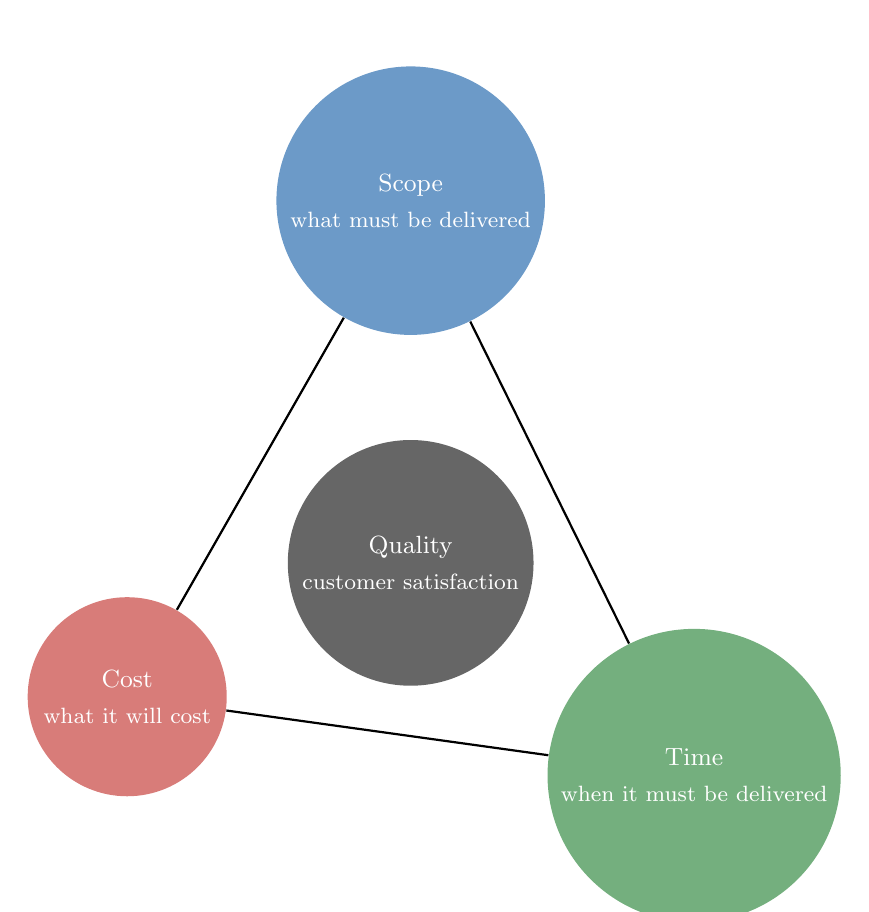
\begin{tikzpicture}[every node/.style={font=\small}]
        \node[circle, fill=myb!70, text=white, minimum size=2cm, align=center] (scope) at (0, 5) {Scope\\[2pt]\footnotesize what must be delivered};
        \node[circle, fill=myg!70, text=white, minimum size=2.4cm, align=center] (time) at (3.6, -2.3) {Time\\[2pt]\footnotesize when it must be delivered};
        \node[circle, fill=myr!70, text=white, minimum size=2.4cm, align=center] (cost) at (-3.6, -1.3) {Cost\\[2pt]\footnotesize what it will cost};
        \node[circle, fill=black!60, text=white, minimum size=2.6cm, align=center] (quality) at (0, 0.4) {Quality\\[2pt]\footnotesize customer satisfaction};
        \draw[thick] (scope) -- (time) -- (cost) -- (scope);
    \end{tikzpicture}
    \caption{The project constraint triad (``iron triangle''): scope, time, and cost surround the central criterion of quality.}
    \label{fig:iron_triangle}
\end{figure}

\begin{prop}[Trade-off Rigidity]\label{prop:trade_off_rigidity}
    Let $S$, $T$, $C$, and $Q$ denote scope, time, cost, and quality, respectively, and suppose the project is executed under fixed total resource availability $R$. Then any admissible change $\Delta S \neq 0$ in scope, holding $R$ fixed, forces a compensating change in at least one of $T$, $C$, or $Q$; that is, no single one of the four factors may be varied in isolation while the remaining three are held exactly constant.
\end{prop}

\begin{proof}
    By \cref{def:project}, the project's resource allocation $R$ is a fixed, finite budget of money, time, and manpower (\cref{pty:uncertainty_characteristics}, item~2). The deliverable quality $Q$ is, empirically, an increasing function of the effort density applied per unit of scope, $Q = Q(S, T, C)$, monotonically non-decreasing in $T$ and $C$ for fixed $S$, and monotonically non-increasing in $S$ for fixed $T$ and $C$ (more scope, same time and cost, cannot increase achievable quality). Suppose $\Delta S > 0$ with $T$ and $C$ held fixed. Since $Q$ is non-increasing in $S$ for fixed $(T,C)$, it follows that $Q(S+\Delta S, T, C) \leq Q(S,T,C)$, with strict inequality generically holding whenever the additional scope consumes finite resources that would otherwise have supported the quality of the original scope. Hence $Q$ must change, contradicting the assumption that all three of $T$, $C$, $Q$ remain constant. The argument is symmetric under variation of $T$ or $C$ instead of $S$.
\end{proof}

\begin{example}[Trade-off in Practice]\label{ex:trade_off_practice}
    If a client requests additional scope (e.g., an additional wing on a building) after the budget and schedule have been fixed, the project manager must either extend the schedule ($\Delta T > 0$), increase the budget ($\Delta C > 0$), or accept a reduction in achieved quality or finish specification ($\Delta Q < 0$) --- precisely the mechanism formalized in \cref{prop:trade_off_rigidity}.
\end{example}

\section{What Is Project Management?}
\label{sec:what_is_pm}

\subsection{Definitions}
\label{subsec:pm_definitions}

\begin{defn}[Management]\label{def:management}
    \textbf{Management} is the process of planning, organizing, controlling, and measuring the use of an organization's resources toward defined objectives.
\end{defn}

\begin{defn}[Project Management]\label{def:project_management}
    \textbf{Project management} is a dynamic process that utilizes the appropriate resources of an organization, in a controlled and structured manner, to achieve clearly defined objectives identified as needs; equivalently, it is the art of directing and coordinating human and material resources throughout the life of a project, using modern management techniques, to achieve predetermined objectives of scope, cost, time, and quality while satisfying all project participants.
\end{defn}

\begin{remark}
    \Cref{def:project_management} combines planning, organizing, staffing, directing, and controlling --- the five classical functions of \cref{def:management} --- and applies them specifically to a temporary, goal-oriented undertaking as characterized in \cref{def:project}. Project management is thus \emph{not} a distinct set of functions from general management, but rather the specialization of general management functions to the boundary conditions imposed by temporariness, uniqueness, and resource constraint (\cref{pty:structural_characteristics,pty:uncertainty_characteristics}).
\end{remark}

\begin{note}
    Project management is always conducted within a defined set of constraints, namely the constraint triad developed in \cref{sec:constraint_triad}. This distinguishes it from open-ended strategic management, in which the constraint set itself may be renegotiated over time.
\end{note}

\subsection{Types of Project Management}
\label{subsec:types_pm}

Project management as a discipline is applied across a broad taxonomy of domains, distinguished by the nature of the deliverable, the regulatory environment, and the dominant risk profile.

\begin{property}[Taxonomy of Project Types]\label{pty:taxonomy_project_types}
    Major categories of project management, as encountered in practice, include:
    \begin{enumerate}
        \item \textbf{Construction projects} --- e.g., bridges, plants, buildings.
        \item \textbf{Manufacturing projects} --- e.g., new production line commissioning.
        \item \textbf{Research and development projects} --- e.g., new material or vaccine development.
        \item \textbf{Information technology (IT) projects} --- e.g., software and systems development.
        \item \textbf{Defence projects} --- e.g., weapons systems, platform acquisition.
        \item \textbf{Healthcare projects} --- e.g., hospital systems, clinical trial logistics.
        \item \textbf{Infrastructure projects} --- e.g., transportation networks, utilities.
    \end{enumerate}
\end{property}

\begin{figure}[H]
    \centering
    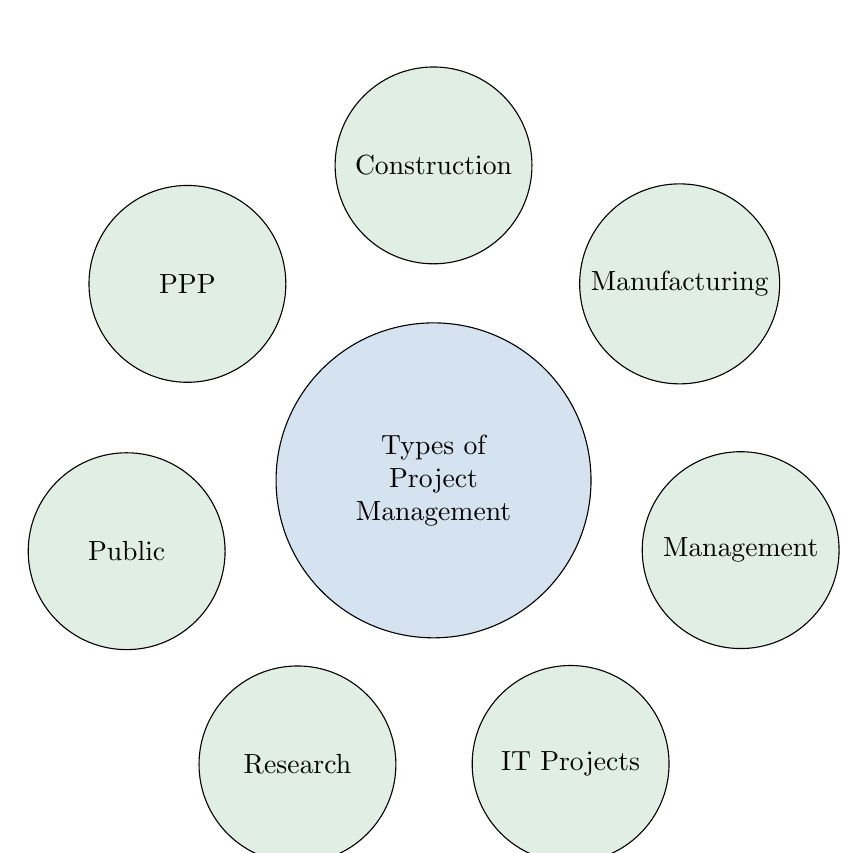
\begin{tikzpicture}
        \node[draw, circle, fill=myb!20, minimum size=4cm, align=center] (core) at (0,0) {Types of\\Project\\Management};
        \foreach \angle/\label in {90/Construction, 38.6/Manufacturing, -12.8/Management, -64.2/{IT Projects}, -115.6/Research, -167/Public, 141.4/PPP}
        {
            \node[draw, circle, fill=myg!15, minimum size=2.5cm, align=center] at (\angle:4) {\label};
        }
    \end{tikzpicture}
    \caption{Radial taxonomy of project management domains (adapted from the lecture figure ``Types of Project Management'').}
    \label{fig:types_pm}
\end{figure}

\subsection{Activities Involved in Project Management}
\label{subsec:activities_pm}

\begin{defn}[Project Management Activity Set]\label{def:pm_activity_set}
    The activity set of project management, denoted $\mathcal{A}_{PM}$, comprises the following operations, exercised iteratively across the project life cycle (\cref{sec:project_life_cycle}):
    \begin{itemize}
        \item Planning and analysing the objectives of the project.
        \item Estimating the organizational resources required.
        \item Assigning tasks to project employees.
        \item Organizing project activities.
        \item Formulating the project (converting objectives into an executable structure).
        \item Measuring and controlling project risk.
        \item Directing and motivating employees.
        \item Forecasting trends in the project.
        \item Completing the project on time.
        \item Maintaining project quality.
    \end{itemize}
\end{defn}

\begin{remark}
    The activities in \cref{def:pm_activity_set} map naturally onto the five classical management functions of \cref{def:management}: planning/estimating/formulating $\to$ planning; assigning/organizing $\to$ organizing; directing/motivating $\to$ directing; measuring/controlling/forecasting $\to$ controlling and measuring.
\end{remark}

\section{The Case for Project Management}
\label{sec:case_for_pm}

\subsection{Need and Importance}
\label{subsec:need_importance}

\begin{prop}[Rationale for Structured Project Management]\label{prop:rationale_pm}
    Structured project management is necessitated by the joint occurrence of the following organizational conditions:
    \begin{enumerate}
        \item Growing size and complexity of undertakings, which renders informal, ad-hoc management unworkable.
        \item Scarcity of resources (money, people, materials), which must be allocated efficiently across competing organizational priorities.
        \item Increasing competitive pressure, which demands faster time-to-market and tighter cost control.
        \item Structural necessity of cross-functional coordination, since no single department can deliver the whole outcome alone.
    \end{enumerate}
    The consequence of applying structured project management under these conditions is a reduction in the probability of cost overruns, schedule slippage, and quality failures relative to unstructured, informal management of the same undertaking.
\end{prop}

\begin{remark}
    \Cref{prop:rationale_pm} explains, historically, \emph{why} project management emerged as a distinct discipline: it arose from the growing demand for complex, sophisticated, customized goods and services, coupled with the exponential expansion of human knowledge, both of which increased the combinatorial complexity of coordination beyond what informal supervisory structures could manage.
\end{remark}

\subsection{Ingredients of Successful Project Management}
\label{subsec:ingredients_success}

\begin{property}[Ingredients of Success]\label{pty:ingredients_success}
    Empirically, successful project management depends on four ingredients:
    \begin{enumerate}
        \item \textbf{Adequate project formulation:} converting the project idea into a structured proposal, avoiding informal, paper-based estimation and overstated projected benefits.
        \item \textbf{Realistic cost and benefit estimates:} avoiding deliberate overestimation of benefits and underestimation of costs.
        \item \textbf{Experienced management:} faulty judgement arising from inexperienced project managers is a leading cause of project failure.
        \item \textbf{Sound integration and control systems:} continuous tracking of status, comparison against the baseline plan, and proactive management of change (formalized in \cref{sec:integrated_project_management}).
    \end{enumerate}
\end{property}

\begin{note}
    Note the asymmetry embedded in item~2 of \cref{pty:ingredients_success}: systematic optimism bias in benefit estimation and systematic underestimation of cost jointly compound, since both errors bias the apparent net present value of the project upward, increasing the probability that a marginal or infeasible project is erroneously authorized.
\end{note}

\subsection{Characteristics of Project Management as a Governance Structure}
\label{subsec:characteristics_pm_governance}

\begin{property}[Governance Characteristics of Project Management]\label{pty:governance_characteristics}
    Project management, viewed as a governance structure, exhibits the following characteristics:
    \begin{enumerate}
        \item The project manager is the single focal point who brings together all resources needed to achieve the objectives, operating outside the normal chain of command.
        \item Because every project requires varied skills, the project manager integrates people from many functional disciplines into a single cohesive team.
        \item The project manager negotiates directly with functional managers for staff and support; conflicts often arise over resource allocation across competing projects and ongoing operations.
        \item A project sits simultaneously inside two chains of command: the vertical (functional) line and the horizontal (project) line.
    \end{enumerate}
\end{property}

This dual-chain-of-command structure, formalized in item~4 of \cref{pty:governance_characteristics}, is the structural origin of the matrix organization commonly used to host projects within functionally organized firms, and is revisited in the treatment of project management structures in subsequent chapters.

\subsection{Case Studies in Practice}
\label{subsec:case_studies}

\begin{example}[Traveler-Tracking at Copenhagen Airport]\label{ex:copenhagen_airport}
    The IT University of Copenhagen collaborated with Copenhagen Airport on a three-year project to improve airport management through traveler-tracking, without invading passenger privacy. The project adopted a unique, low-cost approach: capturing Bluetooth signals emitted by passengers' phones using two electronic readers costing approximately \qty{30}{\$} each. Since only a fraction of passengers carry Bluetooth-emitting devices, the readers provided an effectively random sample sufficient for tracking purposes. To preserve privacy, only a portion of each signal was collected and device addresses were deleted; the public was informed of the project via the airport website and on-site signage, and passengers willing to synchronize their Bluetooth received real-time alerts regarding boarding times and gate directions. This example illustrates the constraint-triad trade-off of \cref{prop:trade_off_rigidity}: a deliberately reduced technical scope (partial signal capture, low-cost hardware) was chosen to satisfy an externally imposed quality constraint (privacy preservation) within a fixed budget.
\end{example}

\begin{example}\label{ex:london_olympic_stadium}
    In 2006, the Olympic Delivery Authority (ODA) selected a one-square-mile, river-surrounded East London disposal site, contaminated with discarded appliances, waste, and soil polluted with petrol, oil, lead, tar, and arsenic, as the location for an 80{,}000-seat stadium with a mid-2011 completion deadline. Project manager Ian Crockford assembled a team exceeding 1{,}000 people, including government employees and stakeholders such as the London Development Agency, politicians, utility firms, community councils, and athlete representatives. Site remediation was performed via an on-site ``Soil Hospital'' staffed by 60 scientists and technicians, processing 800{,}000 tons of soil; surrounding rivers were used for material transport, requiring the dredging of 30{,}000 tons of silt, gravel, and garbage from a waterway that had not seen commercial use in over 35 years. Benchmarking against comparable stadia --- Wembley (90{,}000 seats, 10-year construction) and Sydney's 2000 Olympic stadium (80{,}000 seats, but requiring a footprint incompatible with the site) --- the design team specified that only 25{,}000 of the 80{,}000 seats would be permanent, with the remaining 55{,}000 temporary and built solely for the games, enabling a highly compact playing field acceptable to athletes. Construction, begun in May 2008, initially specified a steel-beamed roof later found to generate aerodynamic turbulence over the compact field; the team redesigned a lighter, more flexible roof incorporating 52 tons of scrap metal from confiscated London police contraband (old keys, knives, and guns), consistent with the ODA's recycled-materials goals, and using only one-quarter of the steel tonnage used in the 2008 Beijing Olympic stadium. The project remained on track for its mid-2011 deadline at a total cost of \qty{537e6}{\pound}.
\end{example}

\begin{remark}
    \Cref{ex:london_olympic_stadium} exemplifies simultaneously: (i) the uniqueness property of \cref{pty:uncertainty_characteristics}, since no directly comparable stadium existed with an equivalent site footprint; (ii) the stakeholder multiplicity discussed in \cref{sec:project_stakeholders}; and (iii) mid-execution scope revision in response to newly discovered technical risk (the roof redesign), illustrating that the constraint triad of \cref{sec:constraint_triad} must be actively re-balanced throughout execution, not merely at project initiation.
\end{remark}

\section{Project Stakeholders}
\label{sec:project_stakeholders}

\begin{defn}[Project Stakeholder]\label{def:project_stakeholder}
    A \textbf{project stakeholder} is an individual, group, or organization that is actively involved in a project, or whose interests are positively or negatively affected by the project's execution or outcome.
\end{defn}

\begin{example}[Stakeholder Categories]\label{ex:stakeholder_categories}
    Representative stakeholder categories, following the Project Management Institute (PMI) taxonomy, include: customers, users, investors, shareholders, partners, media and press, public authorities, governments, trade groups, community groups, protestors, competitors, special-interest groups, and charities. In the terminology of the source material, canonical examples are the customer, the sponsor, the project manager, the project team, suppliers, government, and society at large.
\end{example}

\begin{note}
    Stakeholder interests need not be aligned: the same project may simultaneously advance the interests of the customer (item delivered) while imposing negative externalities on community groups (construction disruption) or competitors (loss of market share). Stakeholder \emph{management}, distinct from stakeholder \emph{identification} as given in \cref{def:project_stakeholder}, is the process of reconciling these divergent interests within the constraint triad of \cref{sec:constraint_triad}, and is treated more fully in later chapters on project risk and contract management.
\end{note}

\section{Integrated Project Management}
\label{sec:integrated_project_management}

\subsection{The Systems Approach}
\label{subsec:systems_approach}

\begin{defn}[Integrated Project Management]\label{def:integrated_project_management}
    \textbf{Integrated project management} is the application of a systems approach to project execution: attention is paid jointly to the goal-oriented system, its environment, its sub-systems, and the relationships among them, such that scope, schedule, cost, quality, resources, communication, and risk are unified into a single coherent plan rather than managed in isolation.
\end{defn}

Formally, a project may be represented as an open system with the following transformation structure:
\begin{equation}
    \text{Inputs (resources)} \;\longrightarrow\; \text{Processes (planning, execution)} \;\longrightarrow\; \text{Outputs (deliverables)} \;\longrightarrow\; \text{Feedback (monitoring \& control)}
    \label{eq:project_system_transformation}
\end{equation}

\begin{remark}
    \Cref{eq:project_system_transformation} closes the loop from outputs back to inputs via a feedback channel, distinguishing integrated project management from a simple open-loop production pipeline: monitored deviations from the baseline plan are fed back into subsequent planning and resource-allocation decisions, consistent with the control-system view developed in \cref{subsec:control_system}.
\end{remark}

\begin{defn}[Project Viewpoint]\label{def:project_viewpoint}
    The \textbf{project viewpoint} is the synthesis obtained by applying classical management principles, behavioural management principles, and systems management principles to the unique requirements of a project as characterized by \cref{def:project}.
\end{defn}

\subsection{The Integrated Project Management Control System}
\label{subsec:control_system}

\begin{defn}[Integrated Project Management Control System]\label{def:control_system}
    An \textbf{integrated project management control system} is a set of software tools, processes, and procedures used to systematize and administer a project as a single coherent whole.
\end{defn}

\begin{property}[Functions of the Control System]\label{pty:control_system_functions}
    The control system defined in \cref{def:control_system} enables management to:
    \begin{enumerate}
        \item Know the current status of the project at any point in time.
        \item Compare actual progress against the baseline (threshold) plan.
        \item Execute and control the change process in a disciplined manner.
        \item Track Earned Value (EV) so as to judge cost and schedule performance objectively.
    \end{enumerate}
\end{property}

\begin{note}
    Item~4 of \cref{pty:control_system_functions} references \emph{Earned Value Management} (EVM), a quantitative technique for jointly assessing cost and schedule performance that is treated in detail in the chapter on project planning and control; it is introduced here only insofar as it constitutes a core function of the integrated control system.
\end{note}

\subsection{Hierarchical Integration: From Strategy to Project}
\label{subsec:hierarchical_integration}

\begin{defn}[Hierarchical Levels of Integrated Management]\label{def:hierarchical_levels}
    Integrated management of projects necessitates combining the following three dimensions under a single organizational-culture and environmental umbrella, each dimension feeding the one above it and receiving governance direction from the one below:
    \begin{enumerate}
        \item \textbf{Project management:} execution-level management of individual, temporary undertakings.
        \item \textbf{Portfolio management:} the coordinated management of a collection of projects to optimize resource allocation across the organization.
        \item \textbf{Strategic alignment:} ensuring the portfolio, and hence each constituent project, advances the organization's overarching strategic goals.
    \end{enumerate}
\end{defn}

\begin{figure}[H]
	\centering
	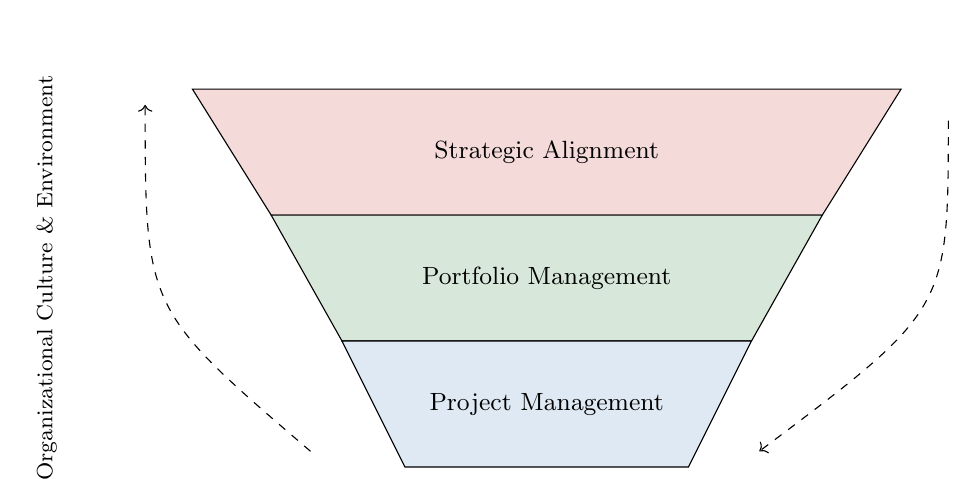
\begin{tikzpicture}[every node/.style={font=\small, align=center}]
		\draw[fill=myr!20] (-4.5,4.8) -- (4.5,4.8) -- (3.5,3.2) -- (-3.5,3.2) -- cycle;
		\node at (0,4.0) {Strategic Alignment};
		\draw[fill=myg!20] (-3.5,3.2) -- (3.5,3.2) -- (2.6,1.6) -- (-2.6,1.6) -- cycle;
		\node at (0,2.4) {Portfolio Management};
		\draw[fill=myb!15] (-2.6,1.6) -- (2.6,1.6) -- (1.8,0) -- (-1.8,0) -- cycle;
		\node at (0,0.8) {Project Management};
		\draw[dashed, ->] (-3,0.2) .. controls (-5.1,2) .. (-5.1,4.6);
		\node[rotate=90, font=\footnotesize] at (-6.35,2.4) {Organizational Culture \& Environment};
		\draw[dashed, ->] (5.1,4.4) .. controls (5.1,2) .. (2.7,0.2);
	\end{tikzpicture}
	\caption{Hierarchical (funnel) integration of project management, portfolio management, and strategic alignment, embedded within organizational culture and environment.}
	\label{fig:hierarchical_integration}
\end{figure}


\begin{property}[Governance under Hierarchical Integration]\label{pty:governance_hierarchical}
    Governance, in the sense of \cref{def:hierarchical_levels}, means applying a set of knowledge, skills, tools, and techniques to a collection of projects in order to move the organization toward its strategic goals. Each dimension of \cref{def:hierarchical_levels} is connected within a single, seamless, integrated domain; this integrative movement represents a major thrust of project-driven organizations across all industries.
\end{property}

\section{The Project Life Cycle}
\label{sec:project_life_cycle}

\subsection{Definition and Motivation}
\label{subsec:life_cycle_definition}

\begin{defn}[Project Life Cycle]\label{def:project_life_cycle}
    The \textbf{project life cycle} is the basic, recurring pattern of change --- a slow beginning, a build-up of size and effort, a peak, a decline, and a termination --- through which every project passes, used to structure planning, budgeting, and control decisions.
\end{defn}

\begin{remark}
    \Cref{def:project_life_cycle} draws an explicit analogy between a project and an organic entity possessing a biological life cycle. The utility of this analogy is not aesthetic but practical: it licenses \emph{phased planning}, whereby decisions are reviewed and re-evaluated at each stage, reducing the risk of committing resources without proper assessment relative to a single, monolithic up-front planning exercise.
\end{remark}

\subsection{The Four-Stage Model}
\label{subsec:four_stage_model}

The project life cycle typically passes sequentially through four stages: \emph{defining}, \emph{planning}, \emph{executing}, and \emph{closing}. The starting point begins the moment the project is authorized (given the go-ahead); project effort starts slowly, builds to a peak, and then declines toward delivery of the project to the customer.

\begin{defn}[Defining Stage]\label{def:defining_stage}
    In the \textbf{defining stage}, specifications of the project are established, project objectives are set, teams are formed, and major responsibilities are assigned.
\end{defn}

\begin{defn}[Planning Stage]\label{def:planning_stage}
    In the \textbf{planning stage}, the level of effort increases, and plans are developed to determine what the project will entail, when it will be scheduled, who will benefit from it, what quality level should be maintained, and what the budget will be.
\end{defn}

\begin{defn}[Executing Stage]\label{def:executing_stage}
    In the \textbf{executing stage}, the major portion of project work --- both physical and mental --- takes place, and the physical product is produced (e.g., a bridge, a report, a software program). Time, cost, and specification measures are used for control: is the project on schedule, on budget, and meeting specifications? What are the forecasts of each of these measures, and what revisions or changes are necessary?
\end{defn}

\begin{defn}[Closing Stage]\label{def:closing_stage}
    The \textbf{closing stage} comprises three activities: delivering the project product to the customer, redeploying project resources, and conducting a post-project review. Delivery may include customer training and the transfer of technical documentation.
\end{defn}

\begin{table}[H]
    \centering
    \caption{Representative activities across the four stages of the project life cycle.}
    \label{tab:life_cycle_stages}
    \begin{tabularx}{\textwidth}{l X X X X}
        \toprule
        & \textbf{Defining} & \textbf{Planning} & \textbf{Executing} & \textbf{Closing} \\
        \midrule
        1 & Goals & Schedules & Status reports & Train customer \\
        2 & Specifications & Budgets & Changes & Transfer documents \\
        3 & Tasks & Resources & Quality & Release resources \\
        4 & Responsibilities & Risks & Forecasts & Evaluation \\
        5 & --- & Staffing & --- & Lessons learned \\
        \bottomrule
    \end{tabularx}
\end{table}

\begin{example}[Life Cycle of a Bridge Construction Project]\label{ex:bridge_life_cycle}
    For the construction of a bridge: the \emph{defining} stage corresponds to identification of the need for the bridge; the \emph{planning} stage corresponds to design and budgeting; the \emph{executing} stage corresponds to the construction work itself; and the \emph{closing} stage corresponds to final inspection and hand-over of the completed bridge to the client.
\end{example}

\subsection{The Six-Phase Extended Model}
\label{subsec:six_phase_model}

A more granular decomposition, applicable in particular to engineering and infrastructure projects with formal contractor engagement, extends the four-stage model of \cref{subsec:four_stage_model} into six phases, arranged cyclically:

\begin{enumerate}
    \item Pre-project phase
    \item Planning and design phase
    \item Contractor selection phase
    \item Project mobilisation phase
    \item Project operations phase
    \item Project close-out and termination phase
\end{enumerate}

\begin{figure}[H]
    \centering
    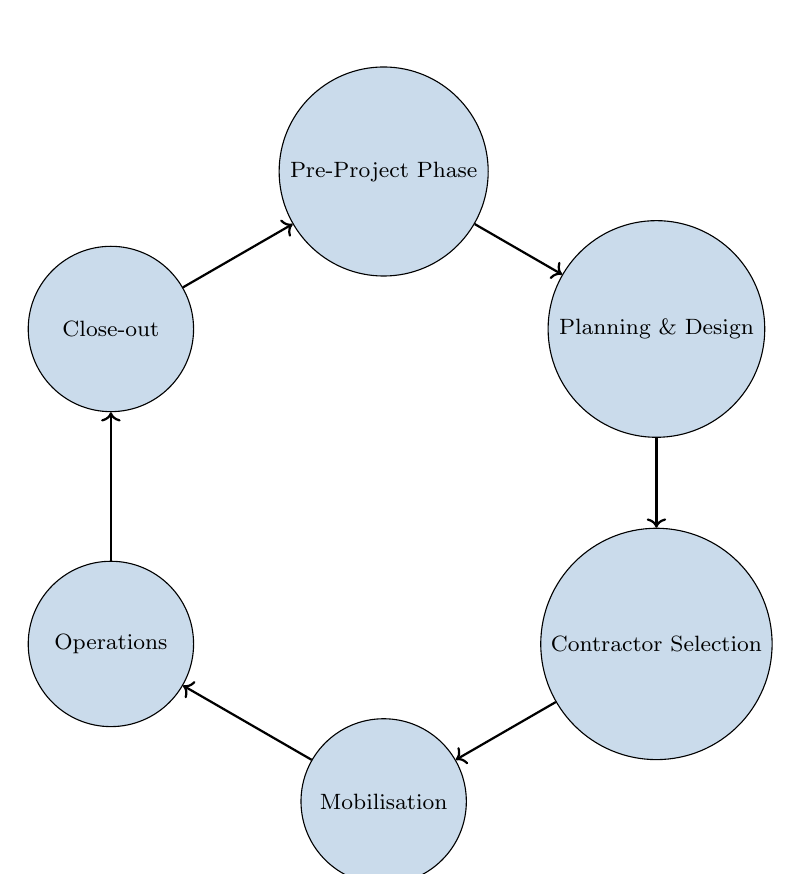
\begin{tikzpicture}
        \foreach \i/\label in {0/{Pre-Project Phase}, 1/{Planning \& Design}, 2/{Contractor Selection}, 3/{Mobilisation}, 4/{Operations}, 5/{Close-out}}
        {
            \node[draw, circle, fill=myb!25, minimum size=2.1cm, align=center, font=\footnotesize] (n\i) at (90-\i*60:4) {\label};
        }
        \foreach \i [remember=\i as \last (initially 5)] in {0,...,5}
            \draw[->, thick] (n\last) -- (n\i);
    \end{tikzpicture}
    \caption{The six-phase extended project life cycle model (cyclic representation).}
    \label{fig:six_phase_life_cycle}
\end{figure}

\subsection{The Stretched-S Effort Curve}
\label{subsec:stretched_s_curve}

\begin{prop}[Stretched-S Shape of Cumulative Effort]\label{prop:stretched_s}
    Let $E(t)$ denote cumulative project effort (measured, e.g., in person-hours or resources expended) as a function of elapsed time $t \in [0, T]$, where $T$ is the total project duration. Under the four-stage model of \cref{subsec:four_stage_model}, $E(t)$ is a monotonically non-decreasing function satisfying $E(0)=0$, $E(T) = E_{\max}$, with:
    \begin{itemize}
        \item $E'(t)$ small for $t$ near $0$ (slow start, corresponding to the defining stage of \cref{def:defining_stage});
        \item $E'(t)$ large and increasing for intermediate $t$ (rapid build-up, corresponding to the transition from planning into execution);
        \item $E'(t)$ decreasing toward $0$ as $t \to T$ (slow finish, corresponding to the closing stage of \cref{def:closing_stage}).
    \end{itemize}
    Consequently the graph of $E(t)$ against $t$ is sigmoidal (``stretched-S'' shaped).
\end{prop}

\begin{proof}[Justification]
    By \cref{def:defining_stage,def:planning_stage}, initial activity is dominated by specification and low-manpower planning tasks, so the rate of resource consumption $E'(t)$ is small. By \cref{def:executing_stage}, the majority of physical and mental project work, and hence the majority of resource consumption, occurs during execution, so $E'(t)$ attains its maximum in this interval. By \cref{def:closing_stage}, closing activities (training, documentation transfer, resource release) consume comparatively little incremental effort relative to execution, so $E'(t) \to 0$ as $t \to T$. A function whose derivative is small--large--small over $[0,T]$, while remaining non-negative and integrating to a finite total $E_{\max}$, necessarily has a graph that is concave near $t=0$, convex-then-concave (inflected) through the middle region, and concave again near $t=T$ --- the defining geometric signature of a sigmoid curve.
\end{proof}

\begin{figure}[H]
    \centering
    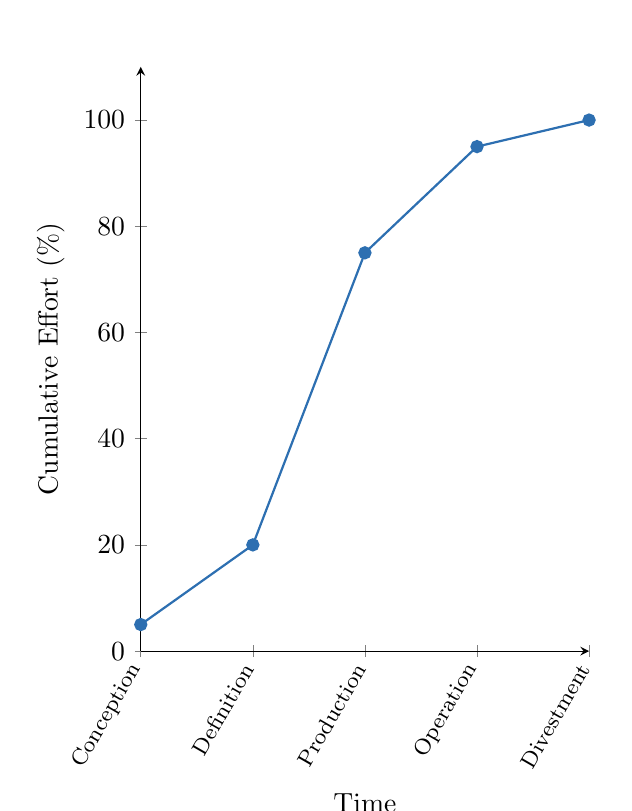
\begin{tikzpicture}
        \begin{axis}[
            width=0.6\textwidth, height=9cm,
            xlabel={Time}, ylabel={Cumulative Effort (\%)},
            xtick={0,1,2,3,4}, xticklabels={Conception, Definition, Production, Operation, Divestment},
            x tick label style={rotate=60, anchor=east, font=\footnotesize},
            ymin=0, ymax=110, ytick={0,20,40,60,80,100},
            axis lines=left,
        ]
        \addplot[myb, thick, mark=*, mark options={fill=myb}] coordinates {
            (0, 5) (1, 20) (2, 75) (3, 95) (4, 100)
        };
        \end{axis}
    \end{tikzpicture}
    \caption{The stretched-S cumulative effort curve: effort builds slowly during conception and definition, rises steeply during production, and tapers off during operation and closeout.}
    \label{fig:stretched_s_curve}
\end{figure}

\begin{remark}
    Not all projects follow the sigmoidal pattern of \cref{prop:stretched_s,fig:stretched_s_curve}. Some project classes, notably software development and chemical-process projects, follow instead a ``J-shaped'' curve, in which most of the observable result appears only near the very end of the project (e.g., a compiled and tested software system provides negligible externally visible value until integration testing is essentially complete).
\end{remark}

\begin{defn}[Instantaneous Effort Curve]\label{def:instantaneous_effort}
    The \textbf{instantaneous effort curve} is the function $e(t) := E'(t)$, representing the level of effort (person-hours or resources expended per unit time, or equivalently the number of people actively working on the project) at time $t$.
\end{defn}

\begin{corollary}[Peak Effort and Derivative Correspondence]\label{cor:peak_effort}
    Under the hypotheses of \cref{prop:stretched_s}, the instantaneous effort curve $e(t) = E'(t)$ attains a single interior maximum (the \emph{peak effort level}) located approximately at the inflection point of $E(t)$, and $e(t) \to 0$ as $t \to 0^+$ and as $t \to T^-$.
\end{corollary}

\begin{proof}
    By the first-derivative test, an inflection point of $E(t)$ (a point at which $E''(t)$ changes sign from positive to negative) corresponds exactly to a local maximum of $E'(t) = e(t)$. Since $E(t)$ is small-slope near $t=0$ and near $t=T$ by \cref{prop:stretched_s}, $e(t)$ is small at both endpoints, and since $E(t)$ has a unique inflection region (the rapid build-up phase) under the four-stage model, $e(t)$ attains a single interior peak, establishing the corollary.
\end{proof}

\begin{figure}[H]
	\centering
	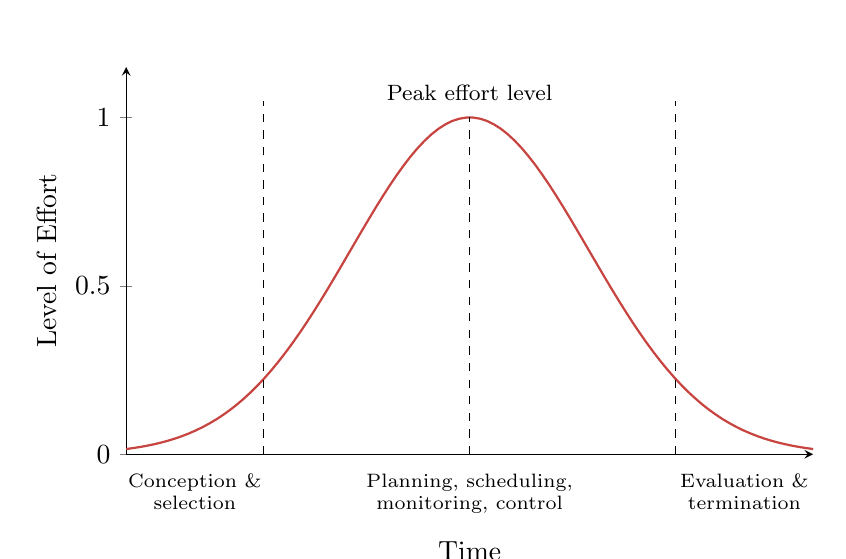
\begin{tikzpicture}
		\begin{axis}[
			width=0.85\textwidth, height=6.5cm,
			xlabel={Time}, ylabel={Level of Effort},
			xmin=0, xmax=10, ymin=0, ymax=1.15,
			axis lines=left,
			xtick=\empty,
			clip=false,
			xlabel style={yshift=-2.6em},
			]
			\addplot[myr, thick, domain=0:10, samples=100] {exp(-((x-5)^2)/6)};
			\draw[dashed] (axis cs:2,0) -- (axis cs:2,1.05);
			\draw[dashed] (axis cs:5,0) -- (axis cs:5,1.0);
			\draw[dashed] (axis cs:8,0) -- (axis cs:8,1.05);
			\node[font=\footnotesize, above] at (axis cs:5,1.02) {Peak effort level};
			\node[font=\scriptsize, align=center, below] at (axis cs:1,-0.03) {Conception \&\\selection};
			\node[font=\scriptsize, align=center, below] at (axis cs:5,-0.03) {Planning, scheduling,\\monitoring, control};
			\node[font=\scriptsize, align=center, below] at (axis cs:9,-0.03) {Evaluation \&\\termination};
		\end{axis}
	\end{tikzpicture}
	\caption{Time distribution of project effort $e(t)$, showing the single interior peak effort level, corresponding to \cref{cor:peak_effort}.}
	\label{fig:effort_distribution}
\end{figure}

\begin{remark}
    Since $e(t)$ is generally non-symmetric about its peak (the rise into peak effort is typically faster than the tail-off, reflecting rapid mobilization but gradual demobilization of resources), the cumulative curve $E(t)$ is likewise non-symmetric, and the location of the inflection point of $E(t)$ need not coincide with the temporal midpoint $t = T/2$.
\end{remark}

\subsection{Characteristics of the Project Life Cycle}
\label{subsec:life_cycle_characteristics}

\begin{property}[Characteristics of the Project Life Cycle]\label{pty:life_cycle_characteristics}
    The project life cycle possesses the following two structural characteristics:
    \begin{enumerate}
        \item The life cycle serves to define the \emph{beginning} and the \emph{end} of a project. For example, when an organization identifies an opportunity to which it would like to respond, it will often authorize a needs assessment or feasibility study to decide whether it should undertake the project.
        \item The project life-cycle definition determines whether the feasibility study is treated as the first phase of the project itself, or as a separate, standalone project preceding formal authorization.
    \end{enumerate}
\end{property}

\begin{figure}[H]
	\centering
	\resizebox{\textwidth}{!}{%
		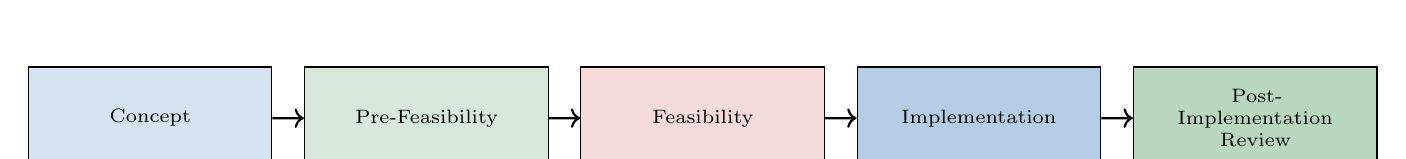
\begin{tikzpicture}[
			stage/.style={draw, trapezium, trapezium left angle=90, trapezium right angle=90,
				trapezium stretches=true, minimum width=3.1cm, minimum height=1.3cm,
				text width=2cm, align=center, font=\scriptsize, inner xsep=2pt},
			node distance=0.4cm,
			]
			\node[stage, fill=myb!20] (c) {Concept};
			\node[stage, fill=myg!20, right=of c] (pf) {Pre-Feasibility};
			\node[stage, fill=myr!20, right=of pf] (f) {Feasibility};
			\node[stage, fill=myb!35, right=of f] (i) {Implementation};
			\node[stage, fill=myg!35, right=of i] (pir) {Post-Implementation Review};
			\foreach \a/\b in {c/pf, pf/f, f/i, i/pir}
			\draw[->, thick] (\a) -- (\b);
	\end{tikzpicture}}
	\caption{Characteristics of the project life cycle: sequential phase-gate progression from concept through post-implementation review, each phase incorporating explicit selection or approval criteria.}
	\label{fig:life_cycle_phase_gate}
\end{figure}


\begin{remark}
    \Cref{pty:life_cycle_characteristics} has a direct practical consequence for project authorization: whether the feasibility study is billed, staffed, and risk-managed as ``project work'' or as a preliminary, separately funded activity is not a universal convention but an organization-specific policy choice embedded in that organization's life-cycle definition.
\end{remark}

\subsection{Why the Life Cycle Concept Matters}
\label{subsec:why_life_cycle_matters}

\begin{prop}[Practical Consequences of the Life Cycle Model]\label{prop:life_cycle_consequences}
    The project life cycle model of \cref{def:project_life_cycle} yields the following practical consequences for project governance:
    \begin{enumerate}
        \item It enables decisions and actions to be taken in structured steps --- the ``phased planning'' approach of \cref{subsec:life_cycle_definition}.
        \item Scope typically takes precedence early in the life cycle (during defining and planning), while schedule and cost dominate as priorities during the main execution stage.
        \item The relative importance of time, cost, and quality shifts across the stages of the life cycle, requiring the project manager to adjust management priorities accordingly.
        \item Recognizing which life-cycle shape applies --- stretched-S (\cref{prop:stretched_s}) versus J-shaped --- is essential to realistic budgeting and scheduling.
        \item Prior to phase-out, senior management conducts a comprehensive evaluation so that lessons learned feed forward into the planning of future projects.
    \end{enumerate}
\end{prop}

\section{The Project Manager}
\label{sec:project_manager}

\subsection{Definition and Role}
\label{subsec:pm_role}

\begin{defn}[Project Manager]\label{def:project_manager}
    The \textbf{project manager} (PM) is the single point of accountability for planning, executing, and closing a project, operating largely independent of the normal functional chain of command and reporting on the project as a whole.
\end{defn}

\begin{property}[Structural Properties of the Project Manager Role]\label{pty:pm_structural_properties}
    The project manager role, as defined in \cref{def:project_manager}, satisfies the following structural properties:
    \begin{enumerate}
        \item The role is inherently cross-functional: the PM must integrate people, technology, and resources drawn from many departments.
        \item Unlike a functional manager, who oversees an ongoing, permanent department, the PM manages a temporary, one-time undertaking with a fixed end date.
    \end{enumerate}
\end{property}

\subsection{Project Manager versus Functional Manager}
\label{subsec:pm_vs_fm}

\begin{table}[H]
    \centering
    \caption{Comparison of the project manager and the functional manager.}
    \label{tab:pm_vs_fm}
    \begin{tabularx}{\textwidth}{l X X}
        \toprule
        \textbf{Aspect} & \textbf{Project Manager} & \textbf{Functional Manager} \\
        \midrule
        Focus & A single, temporary project & An ongoing department \\
        Authority & Often limited, cuts across functions & Full authority within the department \\
        Team & Temporary, borrowed from functions & Permanent staff \\
        Time horizon & Fixed --- ends when project ends & Continuous \\
        Success measure & Scope, time, cost, quality of one project & Ongoing departmental performance \\
        Reporting & Horizontal, project-based & Vertical, functional \\
        \bottomrule
    \end{tabularx}
\end{table}

\begin{example}[Organizational Charts: Functional versus Project Reporting]\label{ex:org_charts_pm_fm}
    In a purely functional structure, a Vice President of Manufacturing supervises functionally organized sub-units --- Welding, Assembly, Machining, and Painting --- each reporting vertically. In a project-based structure, a project manager instead draws horizontally on multiple functional resource pools --- Finance, Engineering, Contracts, Manufacturing, Planning, and Purchasing --- for the duration of a single project, illustrating the dual-chain-of-command property established in item~4 of \cref{pty:governance_characteristics}.
\end{example}

\subsection{Responsibilities of the Project Manager}
\label{subsec:pm_responsibilities}

The responsibilities of the project manager bifurcate naturally into obligations owed \emph{upward and outward} (to the firm and to the client) and obligations owed \emph{inward} (to the project team).

\begin{property}[Responsibilities to the Organization and the Client]\label{pty:pm_responsibilities_org_client}
    To the organization or firm, the project manager is responsible for: proper use of company resources; timely, accurate reporting to senior management; maintaining the firm's reputation with the client; and adherence to policies, ethics, and procedures. To the project and client, the project manager is responsible for: delivering scope on time and within budget; meeting the technical or quality specification; keeping the client informed of progress and risk; and managing changes through formal change control.
\end{property}

\begin{property}[Responsibilities to the Project Team]\label{pty:pm_responsibilities_team}
    Toward the project team, the project manager is responsible for: building a cohesive, motivated team out of individuals drawn from different functions and backgrounds; being fair in workload distribution, recognition, and performance feedback; protecting team members' career interests even though the project itself is temporary, including helping them transition to their next assignment; resolving interpersonal and inter-departmental conflict quickly, since unresolved conflict erodes trust and morale; and keeping the team ``in the loop'' by communicating openly rather than surprising them with adverse news.
\end{property}

\begin{remark}
    \Cref{pty:pm_responsibilities_org_client,pty:pm_responsibilities_team} together instantiate the stakeholder-management challenge introduced abstractly in \cref{sec:project_stakeholders}: the project manager is simultaneously accountable to at least three distinct stakeholder classes --- the firm, the client, and the team --- whose interests need not coincide, and reconciling these accountabilities under the fixed resource envelope of \cref{prop:trade_off_rigidity} is a defining feature of the role.
\end{remark}

\section{Project Integration Management}
\label{sec:project_integration_management_processes}

\subsection{Definition and Rationale}
\label{subsec:pim_definition}

\begin{defn}[Project Integration Management]\label{def:project_integration_management}
    \textbf{Project integration management} is the knowledge area concerned with unifying, consolidating, and coordinating all other project management processes and activities, ensuring that the various elements of the project --- scope, schedule, cost, quality, resources, and risk --- are properly coordinated as a single whole rather than managed in silos.
\end{defn}

\begin{remark}
    \Cref{def:project_integration_management} operationalizes, at the level of individual project processes, the systems-approach philosophy of \cref{def:integrated_project_management}: whereas \cref{sec:integrated_project_management} establishes \emph{why} a unified view is necessary, project integration management specifies the concrete \emph{processes} that realize that unification.
\end{remark}

\begin{prop}[Necessity of Integration under Trade-off Rigidity]\label{prop:necessity_integration}
    Under the trade-off rigidity established in \cref{prop:trade_off_rigidity}, project integration management is necessary: it involves making trade-offs among competing objectives and alternatives to meet or exceed stakeholder needs and expectations. Absent integration, an individually ``correct'' decision made in isolation within one knowledge area (e.g., accelerating the schedule) can silently damage another area (e.g., cost or quality) without being detected until the damage has already propagated through the project.
\end{prop}

\begin{proof}[Justification]
    By \cref{prop:trade_off_rigidity}, a change in any one of scope, time, or cost, under fixed total resources, necessarily induces a compensating change in at least one of the remaining factors, including quality. If the decision-making authority for schedule, cost, and quality is distributed across independent, non-communicating functional silos, then a schedule-optimal local decision made without visibility into its cost or quality consequence is, by \cref{prop:trade_off_rigidity}, generically \emph{not} globally optimal with respect to the full constraint set; the induced damage to cost or quality is realized regardless of whether it was anticipated by the schedule decision-maker. Integration --- centralizing visibility and trade-off authority in a single coordinating process, per \cref{def:project_integration_management} --- is precisely the mechanism that restores the ability to detect and account for this coupling before it is realized as unplanned cost or quality loss.
\end{proof}

\subsection{Benefits of Project Integration Management}
\label{subsec:pim_benefits}

\begin{property}[Benefits of Project Integration Management]\label{pty:pim_benefits}
    Project integration management yields the following organizational benefits: coordination of all project activities under a single coherent authority; avoidance of duplication of work across functional or process silos; improved quality of decision-making, by \cref{prop:necessity_integration}; better utilization of resources; disciplined control of project changes; and an increased overall project success rate.
\end{property}

\subsection{Processes of Project Integration Management}
\label{subsec:pim_processes}

Project integration management comprises seven canonical processes, applied sequentially and iteratively across the four-stage life cycle of \cref{subsec:four_stage_model}.

\begin{defn}[Develop Project Charter]\label{def:develop_project_charter}
    \textbf{Develop project charter} is the process of producing an official document that formally authorizes the project and grants formal authority to the project manager. The charter includes, at minimum, the project scope, budget, timeline, and identified stakeholders.
\end{defn}

\begin{defn}[Develop Project Management Plan]\label{def:develop_pm_plan}
    \textbf{Develop project management plan} is the process of producing the master document that describes how the project will be executed, monitored, and controlled; it consolidates the outputs of all subsidiary planning processes into a single, internally consistent baseline.
\end{defn}

\begin{defn}[Direct and Manage Project Work]\label{def:direct_manage_work}
    \textbf{Direct and manage project work} is the process of executing the planned activities specified in the project management plan (\cref{def:develop_pm_plan}) and managing the resulting project work.
\end{defn}

\begin{defn}[Manage Project Knowledge]\label{def:manage_project_knowledge}
    \textbf{Manage project knowledge} is the process of capturing, sharing, and using project knowledge throughout the project, so that lessons learned and technical insight generated during execution remain available to the current project and to future undertakings.
\end{defn}

\begin{defn}[Monitor and Control Project Work]\label{def:monitor_control_work}
    \textbf{Monitor and control project work} is the process of measuring project performance against the baseline established in \cref{def:develop_pm_plan} and reporting project status, instantiating the control-system functions of \cref{pty:control_system_functions}.
\end{defn}

\begin{defn}[Perform Integrated Change Control]\label{def:integrated_change_control}
    \textbf{Perform integrated change control} is the formal process used to evaluate, approve, reject, and implement changes to the project scope, schedule, cost, or quality baselines, ensuring that all such changes are assessed jointly for their coupled effect across the constraint triad, per \cref{prop:necessity_integration}.
\end{defn}

\begin{defn}[Close Project or Phase]\label{def:close_project_phase}
    \textbf{Close project or phase} is the process comprising final inspection, formal customer acceptance, financial closure, documentation archiving, and release of the project team, corresponding to the closing stage of \cref{def:closing_stage}.
\end{defn}

\begin{algorithm}[H]
    \caption{Project Integration Management Process Flow}\label{alg:pim_process_flow}
    \begin{algorithmic}[1]
        \Procedure{IntegrateProject}{$\text{opportunity}$}
            \State $\text{charter} \gets$ \Call{DevelopCharter}{$\text{opportunity}$} \Comment{\cref{def:develop_project_charter}}
            \State $\text{plan} \gets$ \Call{DevelopManagementPlan}{$\text{charter}$} \Comment{\cref{def:develop_pm_plan}}
            \While{project not closed}
                \State \Call{DirectAndManageWork}{$\text{plan}$} \Comment{\cref{def:direct_manage_work}}
                \State \Call{ManageProjectKnowledge}{} \Comment{\cref{def:manage_project_knowledge}}
                \State $\text{status} \gets$ \Call{MonitorAndControlWork}{$\text{plan}$} \Comment{\cref{def:monitor_control_work}}
                \If{change request raised}
                    \State $\text{decision} \gets$ \Call{PerformIntegratedChangeControl}{$\text{request}$} \Comment{\cref{def:integrated_change_control}}
                    \If{$\text{decision} = \text{approved}$}
                        \State $\text{plan} \gets$ \Call{UpdateBaseline}{$\text{plan}, \text{request}$}
                    \EndIf
                \EndIf
                \If{$\text{status} = \text{deliverables complete}$}
                    \State \Call{CloseProjectOrPhase}{} \Comment{\cref{def:close_project_phase}}
                \EndIf
            \EndWhile
            \Return $\text{lessons learned}$
        \EndProcedure
    \end{algorithmic}
\end{algorithm}

\begin{remark}
    \Cref{alg:pim_process_flow} makes explicit the closed-loop structure already anticipated in \cref{eq:project_system_transformation}: monitoring output (line~7) feeds into change control (lines~8--11), which in turn updates the executing baseline, before the cycle repeats until the closure condition (line~12) is satisfied. This loop is the operational realization of the systems approach of \cref{def:integrated_project_management}.
\end{remark}

\section{Summary}
\label{sec:chapter1_summary}

This chapter established the conceptual and structural foundations of project management. A \emph{project} was defined (\cref{def:project}) as a temporary, unique, resource-constrained undertaking, structurally and statistically distinct from routine operations (\cref{prop:nonstationarity}, \cref{tab:project_vs_operations}); its defining structural and uncertainty characteristics were catalogued in \cref{pty:structural_characteristics,pty:uncertainty_characteristics}. Every project is governed by the constraint triad of scope, time, and cost, mediated by quality (\cref{fig:iron_triangle}), and it was proved formally that no single constraint may be varied while holding the remaining constraints exactly fixed under a bounded resource envelope (\cref{prop:trade_off_rigidity}).

\emph{Project management} was defined (\cref{def:project_management}) as the specialization of the classical management functions --- planning, organizing, staffing, directing, controlling --- to this constrained, temporary setting, and its taxonomy of application domains (construction, manufacturing, R\&D, IT, defence, healthcare, infrastructure) was enumerated (\cref{pty:taxonomy_project_types}). The organizational necessity of project management was traced to growing undertaking complexity, resource scarcity, competitive pressure, and cross-functional interdependence (\cref{prop:rationale_pm}), and the empirical ingredients of successful project management were identified (\cref{pty:ingredients_success}). Two extended case studies --- Bluetooth-based traveler-tracking at Copenhagen Airport and the construction of London's 2012 Olympic Stadium --- illustrated these principles in operational practice. The concept of a \emph{project stakeholder} (\cref{def:project_stakeholder}) was introduced to formalize the multiplicity of interested parties whose needs the project manager must reconcile.

The chapter then developed \emph{integrated project management} (\cref{def:integrated_project_management}) as a systems-theoretic view of the project (input--process--output--feedback, \cref{eq:project_system_transformation}), supported by an integrated control system (\cref{def:control_system}) tracking status, baseline deviation, change, and earned value (\cref{pty:control_system_functions}), and embedded within a hierarchical governance structure linking project management, portfolio management, and strategic alignment (\cref{def:hierarchical_levels}, \cref{fig:hierarchical_integration}). The \emph{project life cycle} was formalized through the four-stage model --- defining, planning, executing, closing (\cref{def:defining_stage,def:planning_stage,def:executing_stage,def:closing_stage}) --- and the extended six-phase model (\cref{subsec:six_phase_model}); the characteristic stretched-S shape of cumulative project effort was proved (\cref{prop:stretched_s}) and its corresponding single-peaked instantaneous effort curve derived (\cref{cor:peak_effort}), with the J-shaped alternative noted for software and chemical-process projects.

The \emph{project manager} was defined as the single point of accountability operating across a dual (vertical/horizontal) chain of command (\cref{def:project_manager}, \cref{pty:pm_structural_properties}), distinguished from the functional manager along focus, authority, team permanence, time horizon, and reporting structure (\cref{tab:pm_vs_fm}), with responsibilities enumerated toward the firm and client (\cref{pty:pm_responsibilities_org_client}) and toward the project team (\cref{pty:pm_responsibilities_team}). Finally, \emph{project integration management} was formalized as the knowledge area unifying all other project processes (\cref{def:project_integration_management}), its necessity was proved as a direct corollary of constraint-triad trade-off rigidity (\cref{prop:necessity_integration}), and its seven constituent processes --- charter development, management plan development, direct and manage work, manage project knowledge, monitor and control work, integrated change control, and project or phase closure --- were formalized and assembled into a closed-loop process flow (\cref{alg:pim_process_flow}). These foundations --- project definition, the constraint triad, the life cycle, the project manager's role, and integration management --- constitute the prerequisite scaffolding for the treatment of project management structures, organizational culture, and market, technical, and financial analysis developed in the subsequent chapter.

\end{document}